\documentclass[a4paper,12pt]{article}   % papír A4, písmo 12 bodu
\usepackage[utf8x]{inputenc}            %kodovaní UTF-8
\usepackage{ucs}                        %kodovani unicode
\usepackage[czech]{babel}               %podpora cestiny
\usepackage[T1]{fontenc}                %pouzij variantu pisma T1 (hacky, carky)
\usepackage[left=2.5cm,right=1.5cm,top=2.5cm,bottom=2.5cm]{geometry} %okraje stranky
\usepackage{amsmath,amsfonts,amssymb}   %podpora matematiky
\usepackage{gensymb,marvosym}           %symboly celsius (\celsius) apod.
%\usepackage{mathptmx}                   %font Times New Roman s~podporou matematiky
\usepackage{times}                      %font Times New Roman (matematika pismem Computer Modern) 
\usepackage{parskip}                    %mezera mezi odstavci
%\usepackage[document]{ragged2e}         %text zarovany vlevo
\usepackage[none]{hyphenat} \sloppy     %slova nedelit a~nepretekat
\usepackage{titlesec}
\setcounter{secnumdepth}{4}
\clubpenalty 10000                      %kontrolovat sirotky
\widowpenalty 10000                     %kontrolovat vdovy
\usepackage{setspace} \onehalfspacing   %podpora pro zmenu radkovani + radkovani 1,5
\usepackage{enumerate}                  %podpora pro zmenu cislovani
\usepackage{fancyhdr}                   %vlastni zahlavi a~zapati
\usepackage{graphicx}                   %podpora grafiky
\graphicspath{{materialy/}}                   %vychozi adresar s~obrazky
\usepackage{caption}                    %popisky
\usepackage{subcaption}                 %podpopisky
\usepackage{siunitx}
\usepackage{MnSymbol,wasysym}
\usepackage[shortlabels]{enumitem}
\usepackage{amsmath}
\usepackage{lastpage}                   %zjištění poslední stránky \pageref{LastPage}
\usepackage{float}                      
\usepackage{url}
\usepackage[unicode]{hyperref}          %klikaci odkazy v~textu
\usepackage{mhchem}
\usepackage{multirow}

\usepackage{halloweenmath}


\titleclass{\subsubsubsection}{straight}[\subsection]
\newcounter{subsubsubsection}[subsubsection]
\renewcommand\thesubsubsubsection{\thesubsubsection.\arabic{subsubsubsection}}
\renewcommand\theparagraph{\thesubsubsubsection.\arabic{paragraph}} % optional, useful if paragraphs are to be numbered


%------------------------ čtvrtá a~pátá úroveň nadpisu ---------------------------

\titleformat{\subsubsubsection}
  {\normalfont\normalsize\bfseries}{\thesubsubsubsection}{1em}{}
\titlespacing*{\subsubsubsection}
{0pt}{3.25ex plus 1ex minus .2ex}{1.5ex plus .2ex}

\makeatletter

\renewcommand\paragraph{\@startsection{paragraph}{5}{\z@}%
  {3.25ex \@plus1ex \@minus.2ex}%
  {-1em}%
  {\normalfont\normalsize\bfseries}}
\renewcommand\subparagraph{\@startsection{subparagraph}{6}{\parindent}%
  {3.25ex \@plus1ex \@minus .2ex}%
  {-1em}%
  {\normalfont\normalsize\bfseries}}
\def\toclevel@subsubsubsection{4}
\def\toclevel@paragraph{5}
\def\toclevel@paragraph{6}
\def\l@subsubsubsection{\@dottedtocline{4}{7em}{4em}}
\def\l@paragraph{\@dottedtocline{5}{10em}{5em}}
\def\l@subparagraph{\@dottedtocline{6}{14em}{6em}}
\makeatother

\setcounter{secnumdepth}{4}
\setcounter{tocdepth}{4}


\setlist[enumerate]{itemsep=0mm}
%_____________________________|___________________________|_____________________________%
%                             |                           |                             %
%-----------------------------| ZDE VYPLNIT UDAJE O PRACI |-----------------------------%
%_____________________________|___________________________|_____________________________%
%                             

\newcommand{\nazev}{Měření amplitudové permeability}                                                        %
\newcommand{\jmeno}{Jakub Dvořák}                                                     %
\newcommand{\datum}{\today}                                                              %
%---------------------------------------------------------------------------------------%


%-----------------------------| POUŽITÁ MAKRA |-----------------------------%

%\newcommand{\zkratka}{ve výsledku se mi napíše tenhle text}
%\newcommand{}{}
%\newcommand{}{}
%\newcommand{}{}
\newcommand{\tsub}[1]{$_\textrm{#1}$}
\newcommand{\texp}[1]{$^\textrm{#1}$}
\newcommand{\tohm}{$\Omega$}
\newcommand{\tmu}{$\mu$}



%_______________________________________________________________________________________%
%_______________________________________________________________________________________%


%----------------------------------- KONEC PREAMBULE -----------------------------------%






%-------------------------------------- DOKUMENT --------------------------------------%
%______________________________________________________________________________________%
\begin{document} %%%%%%%%%%%%%%%%%%%%%%%%%%%%%%%%%%%%%%%%%%%%%%%%%%%%%%%%%%%%%%%%%%%%%%%

\setcounter{page}{0} %cislo strany
\pagestyle{empty} %stranku necislovat

%prostredi pro grafy a~schemata \begin{graf} \begin{schema}
\newfloat{schema}{htbp}{schema}\floatname{schema}{Schéma}
\newfloat{graf}{htbp}{graf}\floatname{graf}{Graf}

\begin{titlepage}
    \begin{center}
        \vspace*{1cm}
            
        \Huge
        \textbf{\nazev}
            
        \vspace{0.5cm}
        \LARGE
            
        \vspace{1.5cm}
            
        \textbf{\jmeno}
            
        \vfill
            
        \vspace{0.8cm}
            
        \Large
            
        \datum\\
        \vspace*{.5cm}
        
\includegraphics[width=.4\textwidth]{logo-cvut-fee.png}\\
    \end{center}
\end{titlepage}

% --- definice zapati a~cislovani ---
\newpage 
\pagestyle{fancy}                                       %vlastni zahlavi/zapati
\renewcommand{\headrulewidth}{0pt}                      %bez linky v~zahlavi
\renewcommand{\footrulewidth}{.5pt}                    %linka v~zapati - optional
\lhead{}       \chead{} \rhead{\nazev}                        %pole zahlavi (prazdna)
\lfoot{\jmeno} \cfoot{} \rfoot{\thepage}   %pole zapati


%------------------------------------ VLASTNÍ TEXT ------------------------------------%



\section{Úkol měření}
\label{chap:ukol}
\begin{enumerate}
    \item 
    \begin{enumerate}[label=\alph*)]
        \item V zapojení na \ref{fig:schema} zobrazte na osciloskopu dynamickou hysterezní smyčku prstencového vzorku magneticky měkkého materiálu při napěťovém magnetování (sinusovém průběhu $B$). Smyčka je zadána maximální hodnotou magnetické indukce $B_\text{m}$. Pozorujte vliv velikosti integrační konstanty použitého pasivního integračního RC článku na tvar smyčky a pro další měření rozhodněte, který z rezistorů R\tsub{1}, R\tsub{2}, R\tsub{3} v integračním článku je vhodné použít.
        \item Z naměřených hodnot $I_\text{1m}$ a zadaných parametrů vzorku určete maximální hodnotu intenzity magnetického pole $H_\text{m}$. Dále pomocí osciloskopu zjistěte hodnotu remanence $B_\text{r}$ a koercitivity $H_\text{c}$.
        \item Změřte závislost amplitudové permeability $\mu_\text{a}$ na maximální hodnotě magnetické indukce pro $B_\text{m}$ = 0,1; 0,4; 0,7; 0,9; 1,1; 1,4; 1,7~T a závislost vyneste do grafu.
    \end{enumerate}
\end{enumerate}

\begin{figure}
  \centering
  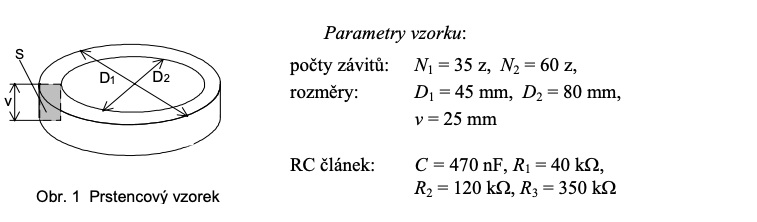
\includegraphics[width=\textwidth]{prstenec.png}
\end{figure}


\section{Schéma zapojení}
\label{chap:schema_zapojeni}
\begin{figure}[h!]
  \centering
  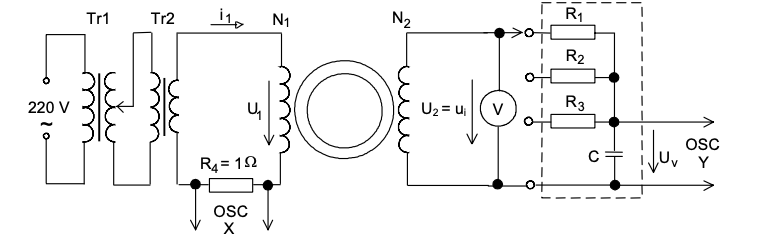
\includegraphics[width=\textwidth]{schema.png}
  \caption{Schéma zapojení pro měření amplitudové permeability a zobrazení dynamické hysterezní smyčky na osciloskopu}
  \label{fig:schema}
\end{figure}


\section{Seznam použitých přístrojů}
\label{chap:seznam_pristroju}
\begin{table}
  \begin{center}
    \begin{tabular}{rl}
      OSC & osciloskop \textit{Keysight}\\
      TR & toroidní transformátor\\
      U & zdroj napětí\\
      RC & integrační článek\\
    \end{tabular}
  \end{center}
  \caption{Seznam použitých přístrojů}
\end{table}


\section{Teoretický úvod}
\label{chap:teoreticky_uvod}
Sice platí velice zjednodušený vztah $H=\mu_O\mu_rB$ nicméně se jedná o velmi nepřesnou stacionární aproximaci Při časové změně magnetické indukce $H$ je odezva magnetického pole $B$ opožděná a "pamatuje si", v jakém stavu byla. Proto vzniká tzv. hysterezní smyčka.
\begin{figure}
  \centering
  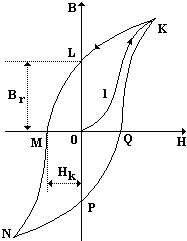
\includegraphics[width=.3\textwidth]{hyst.png}
  \caption{Hysterezní smyčka}
\end{figure}


\section{Naměřené hodnoty}
\label{chap:namerene_hodnoty}


Naměřené hodnoty jsou zanesené v tabulce níže
\begin{table}[h!]
  \centering
  \begin{tabular}{|c|c|c|}
  \hline
  $B_m$ [T] &$U_\text{2} [V]$& $I_m$ [mA]\\\hline\hline
  0,1 & 0,58  & 24   \\ \hline
  0,4 & 2,33  & 70   \\ \hline
  0,7 & 4,07  & 90   \\ \hline
  0,9 & 5,24  & 110  \\ \hline
  1,1 & 6,41  & 130  \\ \hline
  1,4 & 8,15  & 215  \\ \hline
  1,7 & 9,91  & 1550 \\ \hline
  \end{tabular}
\end{table}
$U_2$ spočítáme jako
\begin{equation}
  U_2 = B_m\cdot 4,44 \cdot f\cdot N_2\cdot S_Fe
\end{equation}

\section{Zpracování naměřených hodnot}
\label{chap:zpracovani_hodnot}

Po vyzkoušení jednotlivých rezistorů v integrátoru a optické kontrole průběhu na osciloskopu je zřejmé, že nejlepší ze tří dostupných je $\text{R}_\text{3}$. Jeho velikost je nejvyšší.

\begin{equation}
  \begin{split}
    \frac{H_m}{H_c} &= \frac{X_2}{X_1} ~~\rightarrow~~H_c = \frac{X_1}{X_2}\cdot H_m = 1,56~\text{A}\cdot\text{m}^\text{-1}\\
    \frac{B_m}{B_r} &= \frac{Y_2}{Y_1} ~~\rightarrow B_r = \frac{Y_1}{Y_2}\cdot B_m = 1,5~\text{T}\\
  \end{split}
\end{equation}

\begin{equation}
  H_m = \frac{N_1\cdot I_m}{\pi (D_1 + D_2)} = \frac{35 \cdot 1,55}{\pi (80\cdot 10^{-3} + 45\cdot 10^{-3})} \approxeq 136~\text{A}\cdot\text{m}^{-1}
\end{equation}
Amplitudovou permeabilitu následně spočítáme jako 
\begin{equation}
  \mu_a=\frac{B_m}{\mu_0 H_m} \approxeq 9953
\end{equation}


\section{Závěrečné vyhodnocení}
\label{chap:zaver}
Ze závislosti amplitudové permeability vzorku na ma maximální magnetické indukci je zřejmé, že průběh je nelineární. Velikost $\mu_a$ dosahuje maxima přibližně mezi $1$~T. Pro výběr vhodného rezistoru jsme se řídili podmínkou $\omega RC >> 1$


%--- LITERATURA a~ZDROJE (povinne) ---
\clearpage
\renewcommand{\refname}{Seznam použité literatury a~zdrojů informací} 
%\section*{Seznam použité literatury a~zdrojů informací}
\phantomsection %pridej odkaz do PDF zalozek
\addcontentsline{toc}{section}{Seznam použité literatury a~zdrojů informací}

\begin{thebibliography}{99}

%----------------------------------------------------
\subsection*{Seznam použitých internetových zdrojů}
    \bibitem{navod} Návod k~laboratorní úloze
    
\end{thebibliography}

\end{document}